\chapter{StreamFS System Architecture}
\label{chap:SFSArchMain}

%extendible: able to add and remove stuff 
%scalable: able to scale with applications, data, and deployment size
%generalizable: able to accommodate many kinds of analytical/control applications
%ease of management: so many distributed things that it's hard to keep track of where everything lives.


\begin{figure}[th!] %htbp
\centering
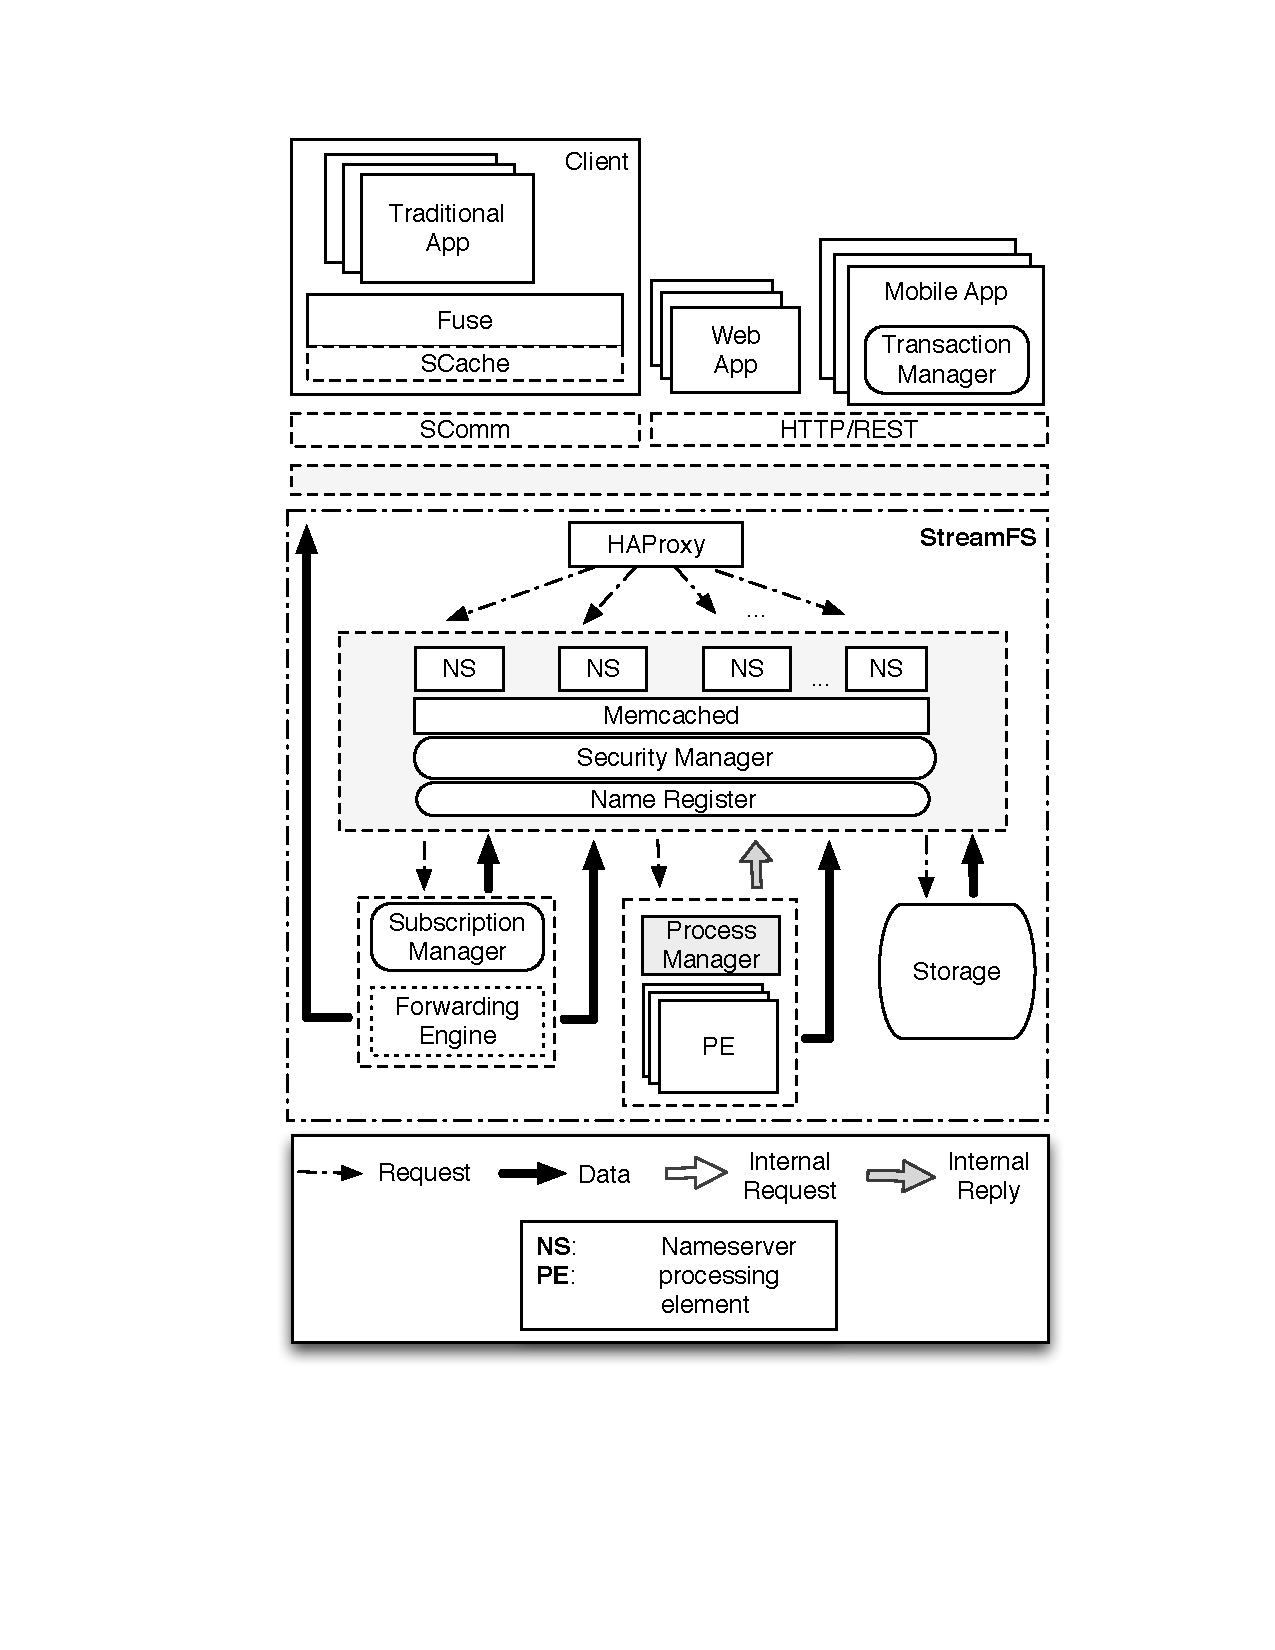
\includegraphics[width=0.65\columnwidth]{figs/sfsarch}
\caption{StreamFS system architecture.  The four main components -- name register, subscription manager/forwarding engine, 
process manager, and timeseries datastore -- are shown.  It also shows the application layer at the top.}
\label{fig:sfsarch}
\end{figure}

StreamFS is a system that addresses some of the shortcomings in the BMS architecture.  StreamFS uses filesystem
constructs to represent \emph{all building information}.  This includes sensors, actuators, location, processing, 
streams, categorical organization, etc.  It borrows several mechanisms used in a Unix-style filesystem: files, folders,
and the pipe abstraction for processing streaming data.  It also employs the principle that \emph{everything is a file} 
that all interactions are through the filesystem.
This eases management of both the raw data and the processing elements that produce derivative streams for further processing.
In this chapter, we give an overview of the architecture -- all the components, their organization, and their interaction.
Throughout this chapter, we refer back to the list in Section~\ref{sec:shortcomings}, where we enumerate the shortcomings
in the design of the BMS architecture in the context of building ``app-ification''.  We also discuss how each component 
provides one or more of the system properties we aim to provide -- extensibility, scalability, generalizability, and
ease of management.


\section{Overview}
Each component in StreamFS addresses the fundamental shortcomings discussed in Chapter~\ref{chap:SensingInBuiltMain}.
The four main components are highlighted below:

\begin{enumerate}

\item \textbf{Name Register}: The name register maintains both the object id namespace and the hierarchical namespace
that it expose to external applications.  It also maintains an entity-relationship graph that is used to support
indirect relationships between objects.  The name register manages various object types as well, which we will discuss
in Chapter~\ref{chap:mechanisms}.

\item \textbf{Subscription Manager and Forwarding Engine}: The subscription manager manages the input stream and output
paths to data-processing sinks.  It is part of the publish-subscribe subsystem.  The forwarding engine is used for internal 
and external data processing.  It queries the
subscription manager and name register to determine where an input datapoint should be forwarded to.

\item \textbf{Process Manager}: The process manager manages the internal and external processes running and managed in StreamFS.

\item \textbf{Timeseries datastore}: The timeseries datastore functions like the NTV storage engine, as discussed in 
Section~\ref{sec:shortcomings}.

\end{enumerate}

StreamFS is built as a web service that resides in the cloud.  It has several interfaces; one is by direct TCP socket communication and 
the other is RESTful~\cite{rest} over HTTP.  We use HAProxy~\cite{haproxy} to scale the service as it grows.  We also design each component
to be horizontally scalable; to grow with the size of the deployment and the number of applications.
Figure~\ref{fig:sfsarch} gives an overview of our architecture as well as the application layer.


\section{Name Management}
The name management layer addresses Point \ref{nw} in Section~\ref{sec:shortcomings}.  It provides a high-level
narrow waist for access sensors in context specified in the name itself.
StreamFS manages two namespaces.  The first is a flat namespaces that identifies a particular
object instance.  The second is a hierarchical namespace that identifies the current instance
of a particular object in some context, specified by the path for the object.  
We support two namespaces in order to uniquely identify sensors and actuators while supporting multiple names.

Supporting multiple names for points in the building is requirement in applications.  Sensors and actuators can be accessed in various 
ways, depending on the application.  Some applications access the sensors in the context of its placement 
in space.  For example, in Soda Hall, the path \texttt{/soda/4F/410/temp} refers to a temperature sensor in room 410.  
The same temperature sensor drives the fans and heating/cooling sub-system in the HVAC system that serves room.
Other applications refer to this sensor through its association to that sub-system.  For example,
\texttt{/soda/hvac/ahu1/temp} gives that contextual information in the name by using a path name that refers to the the specific
air-handling unit in the HVAC system that the temperature sensor drives.
In the rest of this section we discuss how both namespaces are managed and implemented.

\subsection{Object identifier namespace}

When a new object that is created it is assigned a 128-bit unique identifier that uniquely identifier. % the object.
This flat namespace is large enough to support to many objects with low probability of collisions, even across
StreamFS instances.
% Because StreamFS supports multiple names that refer to the same object, we create a namespace that is 
% flat and large enough to uniquely identify objects in the building uniquely.  
% The unique identifier
% is randomly constructed and the probability of collisions is small because of the large namespace.
StreamFS only assigns a unique identifier to stream and control files, since these represent unique channels for a specific 
object in the deployment.  We discuss StreamFS file types in Section~\ref{chap:naming}

% \begin{itemize}
% \item 96 high-order bits identify the object
% \item 32 low-order bits identify the version of the object
% \end{itemize}

% In this paper we concentrate on the high-order bits used to identify the object.  Management of the low-order
% bits is the subject of related, ongoing work.

\subsection{Hierarchical Namespace}

Hierarchical naming schemes are an effective way to organize information, particularly for a relatively small amount of information
where the access patterns are well defined and groups across buildings have a lot of overlap.  For example, upon close examination of
the naming scheme for points across Sutardja Dai Hall, Soda Hall, Cory Hall, and the University of Tokyo Engineering Building 2, we 
observe that there are 2 overlapping group types.  All the point name refer to the location of the sensor and the system that it is 
associated with.  For example, `SODA1R430A\_ART' encodes the name of the building and the room number but also encodes the HVAC subsystem id --
referred to by the 5th character which is a `1'.  The other common encoding include the type of sensor and implies the S.I. units of measure.
Based on our experience with anlysis jobs on building sensor data, we decide it was less import from a naming persepctive than 
an interpretive one.

Because of the number of sensors in the building is on the order of one to ten thousand we adopt the principles articulated 
in~\cite{hierarchy_is_dead}, which asserts that hierarchical organization of files is ineffective when dealing with a large number of files
and that databases are poor at providing direct access to the data, but provide a good way to find the information we are looking for.
We combine these two, as suggested by the authors.  We expose a hierarchical namespace that gives the user direct access to the data
through a familiar organization of that data.  The organization itself is directly traversable.  Moreover, we separate the metadata from
the naming structure, so that users looking for various kinds of information can quickly locate it.

The decision to separate these also gives our implementation \emph{better scalability}.  The growth of the namespace, metadata, and data
happen at different rates.  For example, files and often added and removed, but after creation, changes to the metadata occur less
often that writes to stream file (data produced by sensors).  Moreover, since the 3 kinds of meta/data are accessed in different ways,
we tailor its acquisition to the information being fetched and separate how where/how we store each. % depending on the type of information
%being requested.  
For example, if the query is metadata-related, we send it to the metadata management cluster, which not only stores
the metadata, but also indexes it accordingly.  The data is stored in a time-series database, and the namespaces are stored in a relational
database.  This allows each to grow separately and maximizes fetch efficiency.  Overall, the hierarchical namespaces provides 
\emph{extensibility and ease of management}.
% Because the hierarchical namespace is easily extendable, it provides a natural
% way to group items which eases \emph{management and access}.
We discuss our naming structure in more detail in Chapter~\ref{chap:naming} and give an overview of fundamental challenges that emerge when
naming must reflect physical associations and the physical environment is changing.

\subsection{Implementation Details}

The name management layer is implemented behind HAProxy, an open source load balancer. The implementation includes 
a name registry and a name server.  Several name server handles requests that are forwarded
from HAPRoxy to one of the name servers.  Each of the name server knows of each of the databases that contains names. 
In all our deployments, we only had a single server.  However, for deployments that are large, we put the names in multiple, 
replicated databases with a write-through update policy.  Reads are done from any of the database servers, randomly, since
they all contain the same information.  %Each name server has a preference, so the load is properly distributed.

\begin{figure}[h!] %htbp
\centering
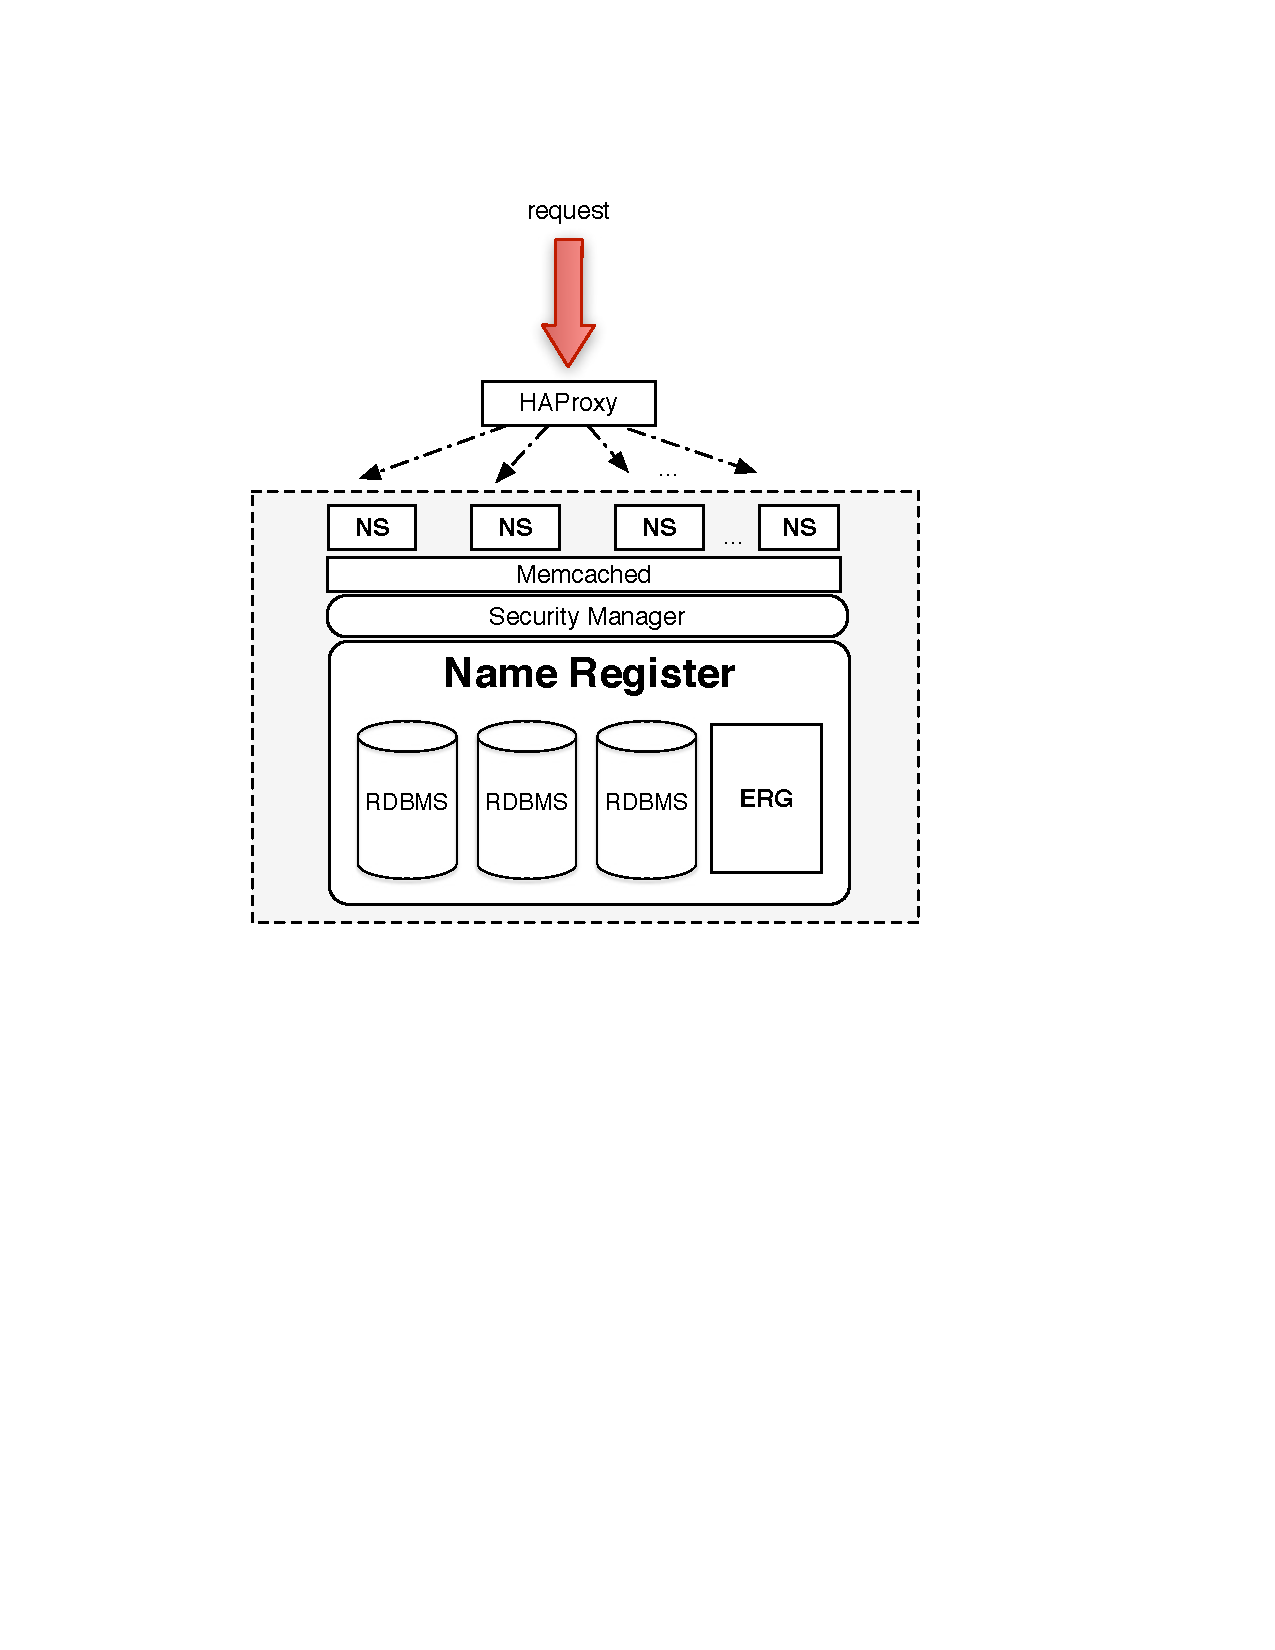
\includegraphics[width=.55\columnwidth]{figs/name_reg}
\caption{Name management layer implemented behind HAProxy.  Name servers handle individual requests and use the name registration table
query handle the request accordingly.}
\label{fig:nameserver}
\end{figure}

The write-through policy is implemented with a write lock.  Whenever a name server receives a request to create or delete a file it informs the
other name servers that it wishes to acquire a lock.  To prevent deadlock, we force a lock-acquisition order.  A lock is not acquired unless every
name server agrees to give up the lock to the requesting name server.  Once the lock is acquired, the name server performs the same write on each
server.  The name server then releases the lock by contacting the other name servers in reverse order.  If a name server has given up a lock
and not received a release, the lock is released automatically after some time.  If a name server goes down, the name server that acquired the lock
assumes the release was successful.  The name server list is immutable, they are restarted in practice if they go down.

A layer of memcached~\cite{memcached} is used to reduce the load on the databases.  Writes immediately invalidate any entries in memcached.  
We also include file metadata in the memcached layer, so its use reduces the load on both the name register and the metadata store.
The security manager essentially maintains an access control list and set of operations that are supported by each file.  By default, 
security is disabled, but some of our deployments do enable it.

The name management layer consists of 3 dependent components, each following the principles of horizontal \emph{scalability}.  The namespaces are
managed in single replicatable, relational database.  The metadata is managed in a separate MongoDB~\cite{mongodb} database, which is itself
shardable.  The data associated with streams is managed in a timeseries database.  We follow the principle of scale-out
in each sub-component, for \emph{scalability}.












\section{Time-series Data Store}

The timeseries data store addresses point \ref{ts} in section~\ref{sec:shortcomings}.
Data collected from sensor is timeseries in nature.  A sensor produces data periodically.  The important aspect of
the stream are the name of the feed, the time the reading was received, and the value for that reading.  There is also
metadata that needs to be stored about the stream.  For example, we want to know what the units of measure are, 
the make/model of the sensor, the date it was installed, any calibration parameters or other information that will help 
the user locate the sensor or interpret it correct.  We actively separate the storage of the metadata from the storage 
of the data.

In constructing a design for the data store, we considered 3 main questions:

\begin{enumerate}
\item What is the typical access pattern or what are the top queries?
\item Should we compress it?
\item How is the data stored long-term?
\end{enumerate}

The typically access pattern is that of scans.  Many of the applications that we consider that make use of historical data, fetch the data
is a temporally meaningful manner.  The query specifies the interval of time over which to fetch the data from a particular feed
and either perform cleaning operations on the data, display it, or adjust the scan parameters for a subsequent query.
The data is largely self-similar and highly compressible.  Simple compression tests we ran on real data showed a compression factor 
between 15 and 30.  Also, the data is essentially append-only, forever.  It can grow quite large, but grows have a fairly 
slow rate, especially after compression.  For example, the total footprint of the SDH deployment, uncompressed 
is nearly 100 GB, however, after compression it is only about 4 GB.
All timeseries data is stored as a 3-tuple that included the name of the stream, a timestamp, and value.  The name we use in
the datastore is the unique id that is generated by StreamFS.  %The human-readable name is fetched

\subsection{Implementation Details}

\begin{figure}[h!] %htbp
\centering
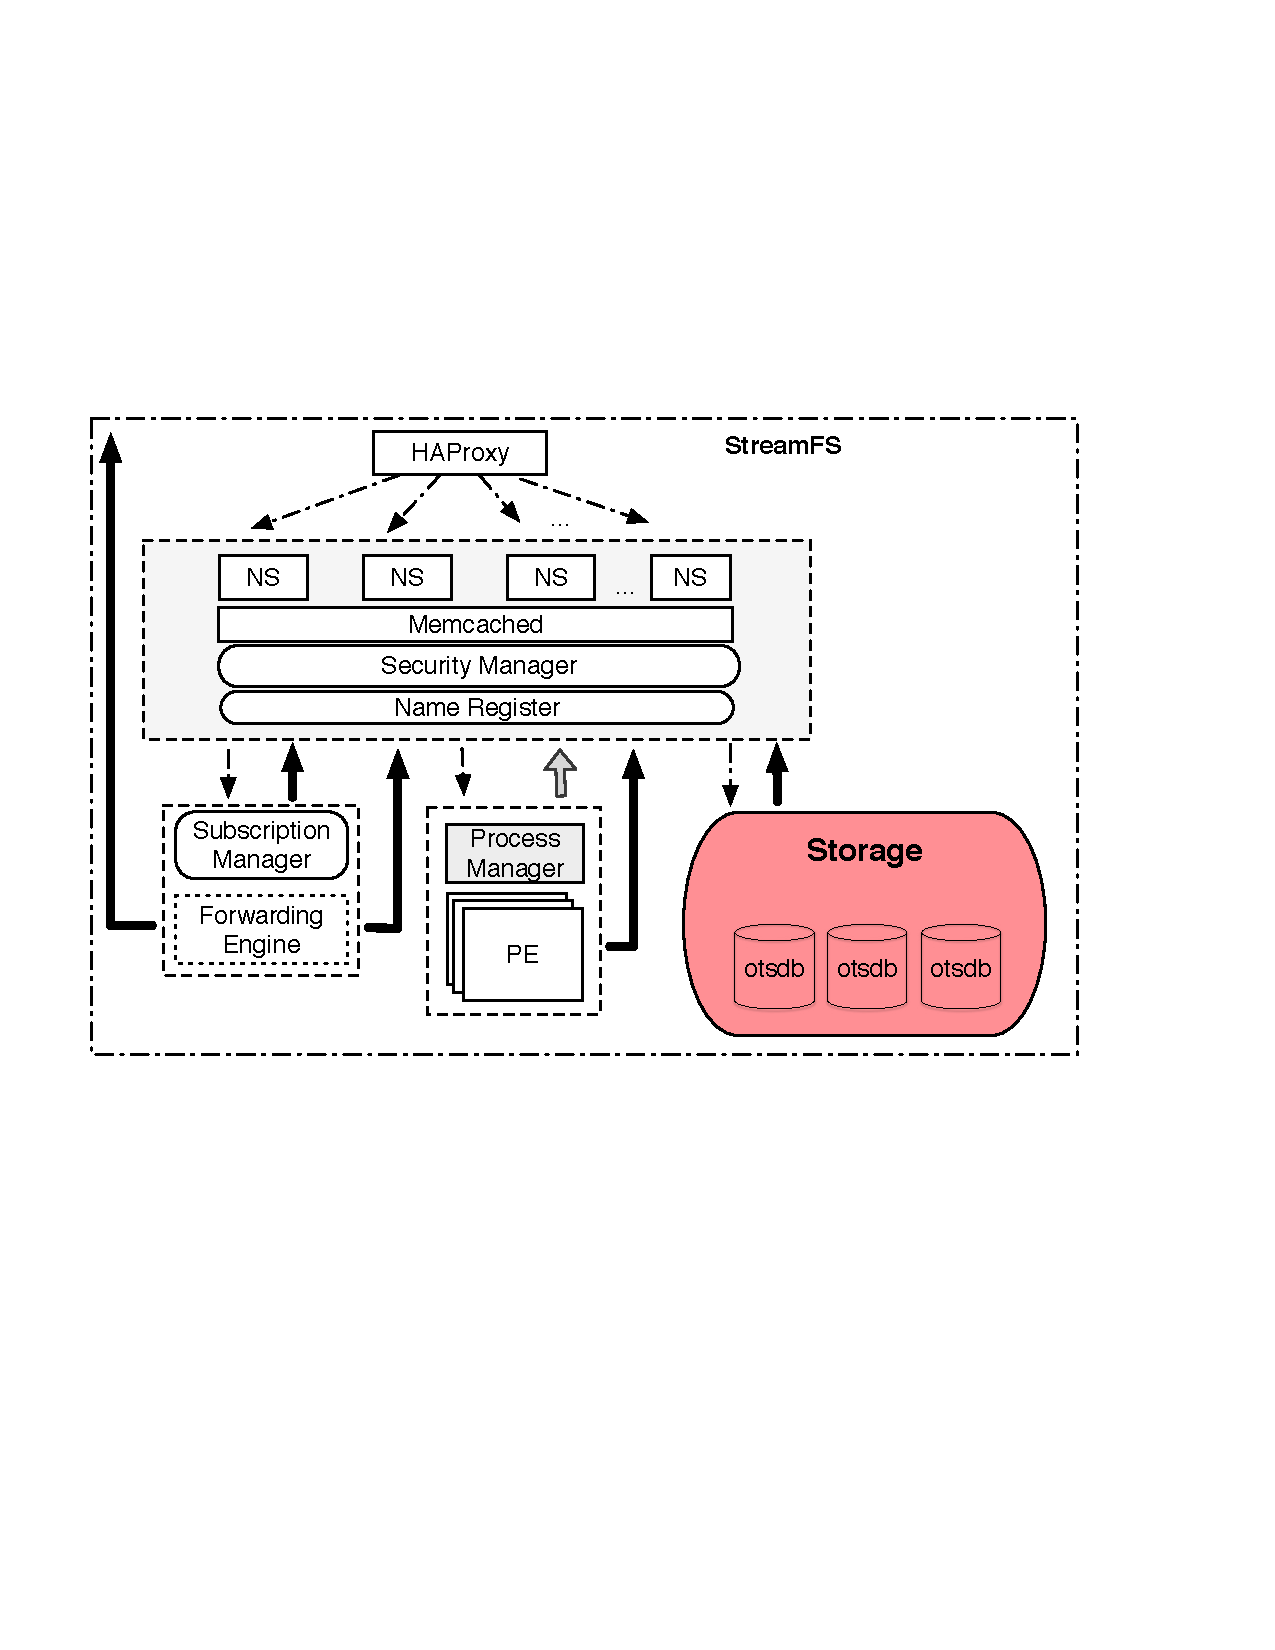
\includegraphics[width=.55\columnwidth]{figs/tsdstore}
\caption{The timeseries data store.  We use OpenTSDB; a timeseries data-store that runs in a cluster setting over
HBase.}
\label{fig:tsdb}
\end{figure}

We use OpenTSDB~\cite{opentsdb} as our primary data store. We enable compression  and index on the name and timestamp 
of the feed.  OpenTSDB is a timeseries data store built on HBase~\cite{HBase}.  HBase is designed to scale horizontally for very
large data sets.  OpenTSDB is a good choice because the compression features keep the footprint small/fast while the append-only 
workload requires a scalable solution.

\section{Publish-Subscribe Subsystem}
\label{sec:ProcMngtSchedMain}

StreamFS uses a flexible construction of the publish/subscribe model in order to support a wide range of applications.
It addresses point \ref{rt} in section~\ref{sec:shortcomings}.  It includes both the process manager and processing
features that support \emph{online analytical processing (OLAP)} processing features.
Publish/subscribe is necessary is physical data application development in order to scale in the number of supported
applications.  The publish/subscribe model used in StreamFS provides mechanisms that enable a flexible combination 
of space and time decoupling that enable StreamFS to support of a wide arrange of application requirements, as described by
Eugster et al.~\cite{eugster}.
Our pub/sub engine is also tightly coupled with the namespaces exposed to users, and this design choice allows an application
to control the space coupling between the publisher and the subscriber (similar to TIBCO~\cite{tibco}).  

\subsection{Space decoupling}
By its very design, space decoupling is achieved.  Publisher do not hold a reference to the subscriber and subscribers do not
hold references to publishers.  However, because of the coupling of a full pathname and an object, subscriptions to topics
expressed as a full pathname refer to the single publisher.  Since we maintain a one-to-one mapping between the
name and an object, only a single stream can fulfill the subscription request.  Space decoupling is achieved when the 
topic is generalized using the star operator in a a regular expression match.  For example, if the user specifies
to obtain all the feeds for \texttt{/soda/4F/*} then all the publishers that have a name that match that prefix will be fowarded
to the subscriber sink.  Space decoupling in achieved because the subscriber and the publishers are unknown.

\subsection{Time decoupling}
Time decoupling is achievable through the timeseries data store.  Publisher push data to StreamFS whether or not subscribers are
online.  Moreover, data may be received at the subscriber even if the publisher becomes disconnected.  Currently, subscribers do
not receive all information that was missed.  In order to achieve fill time-decoupling, we allow the subcription
target to enable or disable the option to buffer all missed readings for an associated subscription target, while the subscription
target it offline.

\subsection{Synchronization decoupling}
Sychronization decoupling is achieved by the publisher and subscribers through StreamFS.  Events are received out of sequence
from their arrival to StreamFS.  This is true even when the subscription target is a processing element.  The thread that buffers
incoming data for each processing element is seperate from the thread where the process is executed.



\subsection{Implementation Details}

\begin{figure}[h!] %htbp
\centering
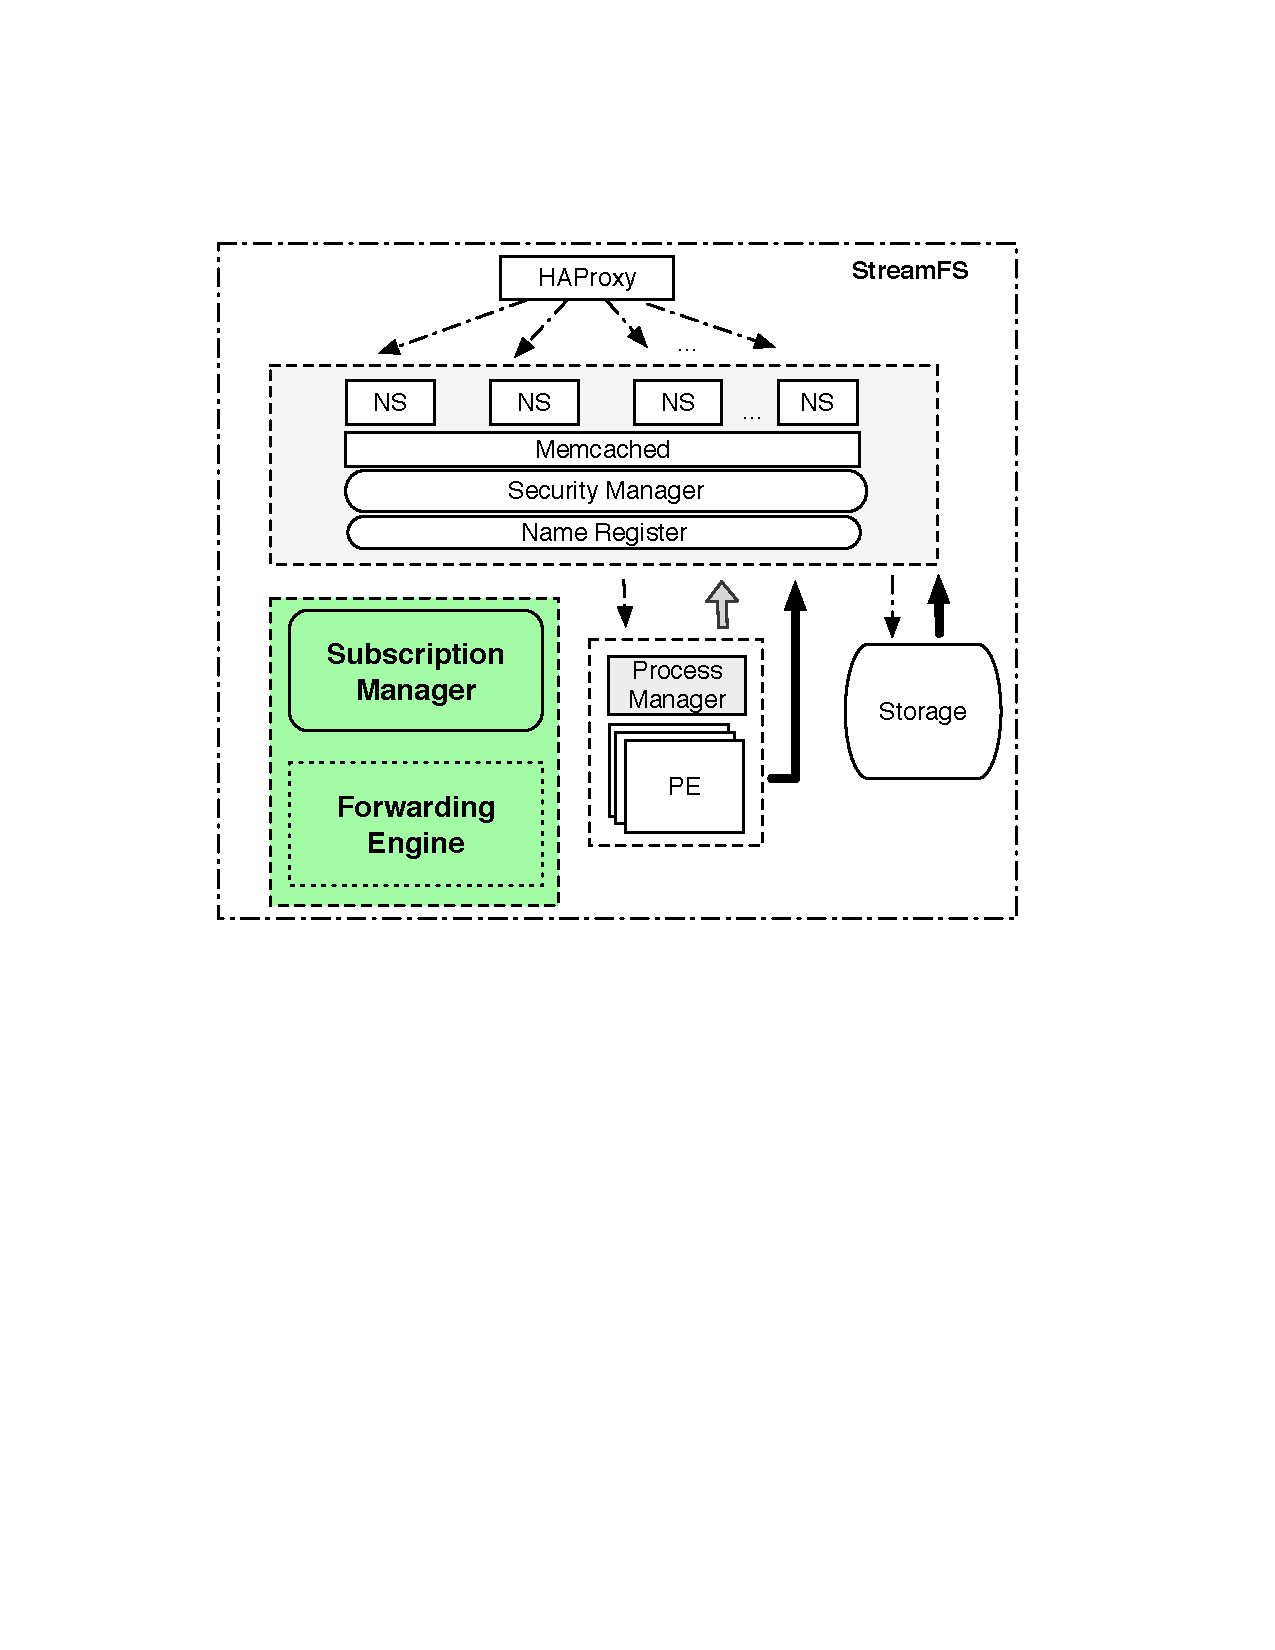
\includegraphics[width=.55\columnwidth]{figs/submngr}
\caption{}
\label{fig:submngr}
\end{figure}

The pub-sub system manager works with the name register to determine where to forward the incoming data.  When data arrives, it arrives
with a tag that contains the name of the publisher.  The subscription manager resolves the name to an object identifier and resolves
all the names for the object.  Then, it scans each of the names and matches them to a subscription.  If the subcription matches \emph{any}
name, the data unit is marked with the subscription id and sends to the forwarding engine.  The forwarding engine then
contact the forwarding sink and send it the data unit.  The subscription sink may be a processing element managed by the process manager.
If so, it is forwarded to the process manager's buffer and the process manager copies it to either an internal buffer for a
process that is running locally or sends it to an external process stub, which copies it in an internal buffer on the client side.
\section{Data Cleaning and Real-time Processing}

Data is coming in at different, independent rate from sensors and is produced asynchronously from internal processing elements.
For certain processes, processing the incoming data as quickly as possible is key, however, this is challenging for several reasons:
1) a process may subscribe to multiple, independent streams with asychronized report schedules and 2) interpolated values
should be avoided to minimize prediction inaccuracies in interpolated values.  Therefore, a process actually wants all the freshest
data from all the streams they are subscribing to, while minimizing the average time that the data for each respective stream has 
been waiting in the buffer.

Sensor data is fundamentally challenging to deal with because much of it must be cleaned before it can be processed.  For example,
it is not uncommon to receive readings that is out of operational range, that is erroneous with respect to the previous observed trend,
or to stop receiving readings altogether.  This implies the need for processing jobs to provide a level of filtering over the raw streams.
Once the data is cleaned, it is typically consumed more sophisticated processes that aggregate the information or use it for control
of the space or equipment.  We provide the mechanisms for handling both classes of processing jobs with our process management layer.
In the next section we will discuss our process management layer and how users can both submit jobs to StreamFS for management or link
their own external processing elements so that they can be managed through StreamFS but run outside of StreamFS.

We also discuss how we deal with the fundamental challenges that come with sensor data.  Specifically, we 
address \emph{re-sampling} and \emph{processing models}.  The incoming data does not have a common
time source, so combining the signals meaningfully involves interpolation.  There are various options that we
provide for performing the interpolation, chosen by the user depending on the units of the data.  For example,
temperature data may involve fitting a heat model with the data to attain missing values in time.  In addition,
aggregation is done as a function of the underlying constituents: they can be combined arbritarily, by adding
subtracting, multiplying or dividing corresponding values.  We provide an interface to the user that
allows them to specify how to combine the aggregate signals as a function of the child nodes in the entity-graph.
Futhermore, they can filter the data by unit.  This kind of flexibility useful for visualizing
energy consumption over time.



\section{Entity-relationship Model}

StreamFS supports symbolic links, which allows the user to specify non-hierarchical relationships.  Indeed, they can 
be used to express relationships which form a directed graph.  We find that many applications, such as control 
applications and applications that perform aggregation, precede their timeseries queries with multiple queries
to determine indirect relationships between streams.  Fundamentally, the queries were use to ascertain a multiple-hop
relationship between streams and could be easily and efficiently answered with a single graph query.
StreamFS maintains an entity-relationship graph (ERG) that uses the names and symbolic links to construct a queryable 
graph.

The ERG is used throughout our architecture; for answering graph queries by the user and for subscription topic-matching.
The latter is slightly different from the topic-matching mechanism traditionally available in pub-sub systems. 
We discuss the details of our approach in section~\ref{sec:ProcMngtSchedMain}.


\subsection{ERG to OLAP}
\label{sec:erg2olap}

Many of the operations that users perform are OLAP-style (online analytical processing) operations\cite{Gray1996}. 
OLAP databases build a logical hypercube along multiple dimensions.  The values in the cells are called 
measures.  Queries makes use of the cube to aggregate data along those dimensions.
We provide OLAP-style queries using the ERG.  This is similar to the work proposed by Chen et al.~\cite{Chen2008_olapgraph}.
The time dimension is fixed, the categorical dimension is determined by the hierarchy, and the unit are specified
by the user.

\begin{figure}[h!] %htbp
\centering
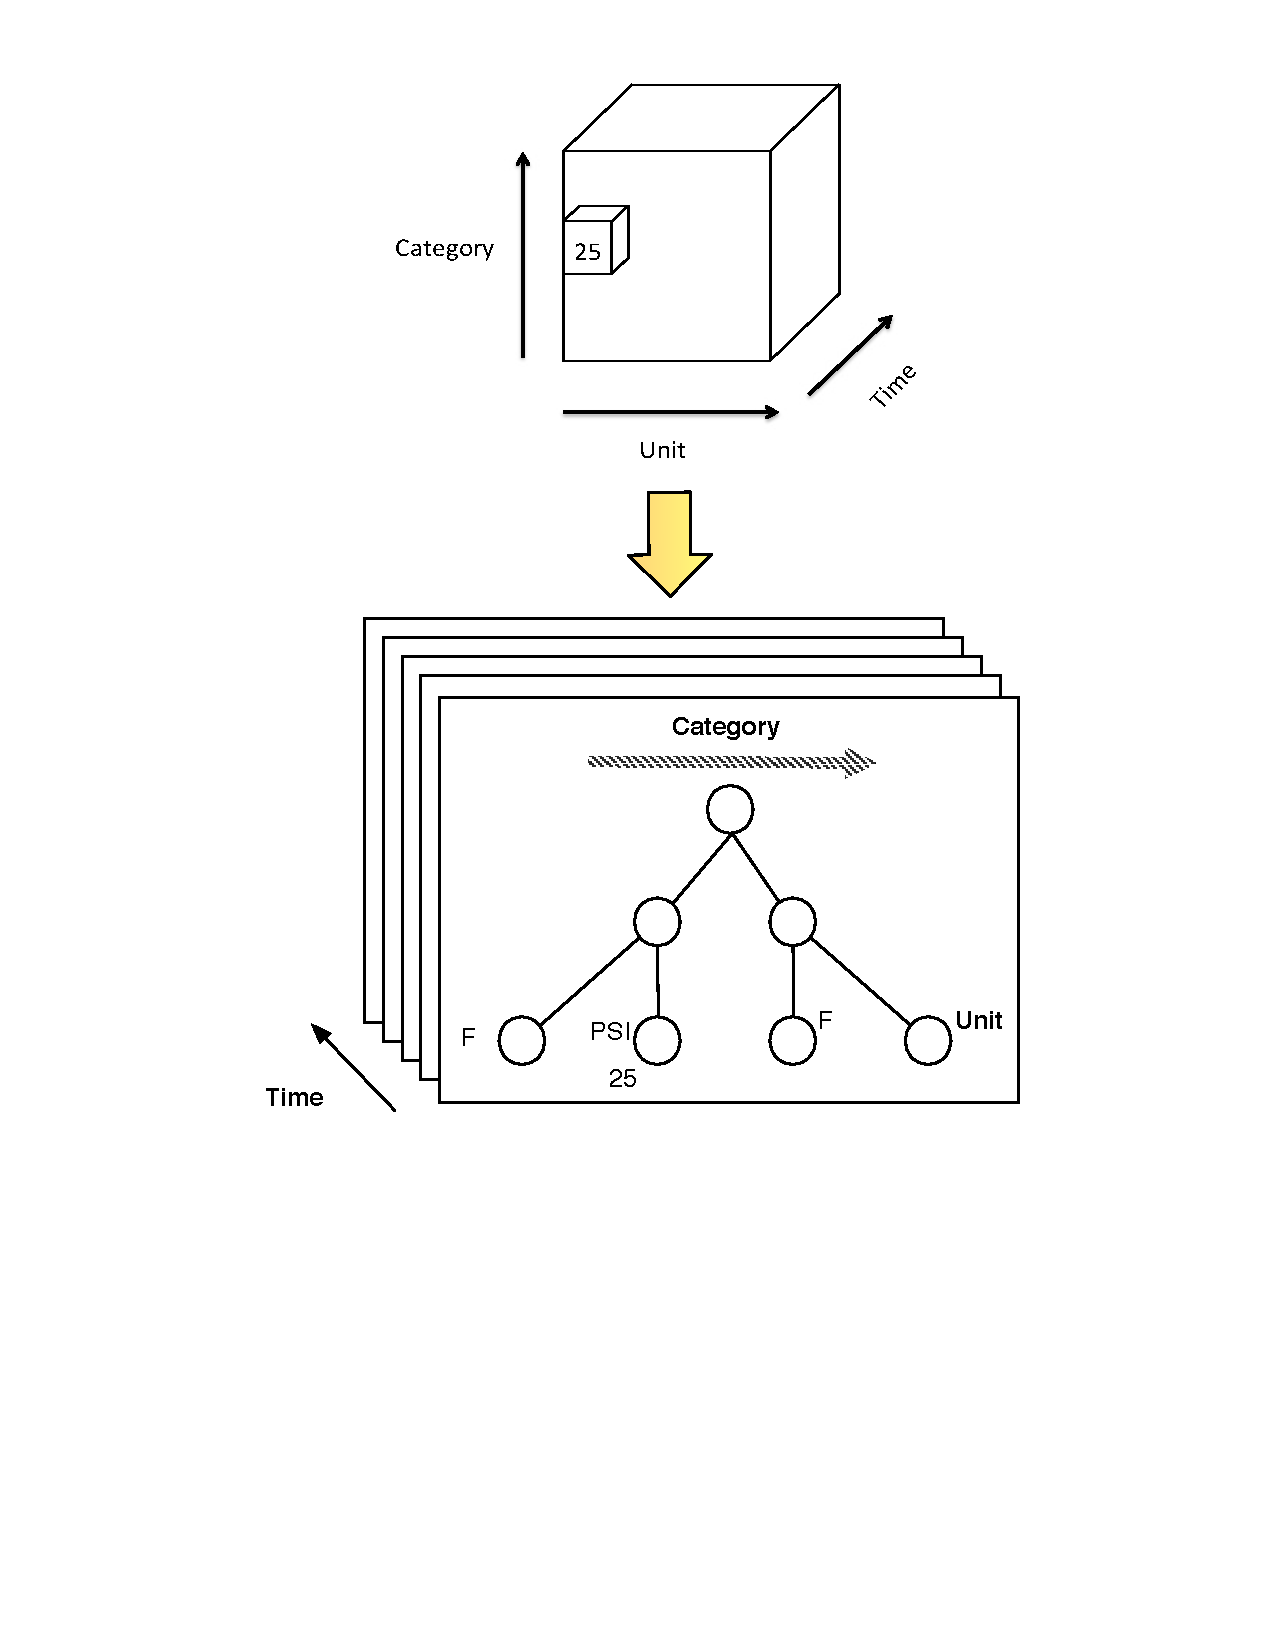
\includegraphics[width=.55\columnwidth]{figs/olaptoerg}
\caption{This figure shows how we translate the OLAP cube to a hierarchical ERG.  Note how the dimensions of the cube translate
to the graph.  The level of the subtree is the category, the unit is specified at the node, and there are values at each node
for every time slice.}
\label{fig:olap2erg}
\end{figure}

% where it can be used more effectively, and how to change the operation of the building -- through better equipment or activity scheduling -- 
% in order to optimize and reduce its energy consumption.
% For building-oriented energy analytics applications the building manager and occupants typically want answers
% to the following set of questions:
Below is a typical list of questions that can be answered efficiently with OLAP-style queries.  

\begin{enumerate}
\item How much energy is consumed in this room/floor/building?  On average?
\item What is the current power draw by this pump? cooling tower? heating sub-system?  Over
		the last month?
% \item How much power is this device currently drawing? Over the last hour?
%\item What percentage of the total building power is being drawn by the plug-load devices? 
% \item How much energy have I consumed today?  Versus yesterday?
\item How much energy does the computing equipment in this building consume?
%\item {\bf For all queries:} What's the trend over time?
\end{enumerate}
\vspace{0.08in}

% Notice, these question span space and time and require aggregation along a dimension, such as power.  
These questions require the ability to answer a series of questions
about energy flow -- energy data aggregated across multiple categories to determine how, where, and the amount used.  
The ability to \emph{slice and dice} the data allows the analyst to gain better insight into how the energy is being used.
Notice how questions translate into categorical and spatio-temporal queries.
There is also a hierarchical grouping characteristic to them.  For example, to answer the first question we must 
aggregate the data from the individual rooms up to the whole building (if the whole building data is not available)
% This hierarchical relationship
% is not as evident in the HVAC sub-components specified in the second question.  However,
% local hierarchically relationships do exist.  For example, 
Also, the cooling system consists of the set of pumps, cooling towers, and condensers in the HVAC system that push condenser
fluid and water to remove heat from spaces in the building.  We can model this as a set of objects and inter-relationships which inform how
to \emph{drill-down}, \emph{roll-up}, and \emph{slice and dice} the data -- traditional OLAP operations.
Figure~\ref{fig:olap2erg} shows how we translate an OLAP cube to a hierarchical arrangement of 
nodes in the ERG.  Time-range queries on any node translates to a slice in the cube along the time dimension.
\emph{Pivoting} along any dimension can be done by taking slices along the ``cube'' in the bottom of that
figure.
% The dynamic aggregation processing model accommodates many common situations where aggregation of feeds is the primary
% objective.  For example, consider a power meter attached to a fan running in a variable air-volume (VAV) unit.
% There can be several hundred VAV units throughout the entire building, one in each space that is controlled by 
% the HVAC system.  An energy auditor may want to determine the energy consumption with respect to either a space 
% or a system or by category.  If these three ``views'' are of interest, there would be three sub-trees in the namespace, 
% rooted at the building: \texttt{/hvac/}\dots\texttt{/vav/fan}, \texttt{/zones/}\dots\texttt{/vav/fan}, 
% and \texttt{/loads/}\dots\texttt{/fans}.  The first is the 
% sub-tree that represents the HVAC sub-components and their inter-connection, the second one describes the set 
% of zones, and the third one is a categorical partitioning of the loads in the building.  With dynamic aggregation,
% as data is received from the each fan stream, it continues up-stream to the aggregation points.
% So, for the total power consumption of the hvac system, you query \texttt{/hvac} (which includes the fans),
% for the total energy consumed in a particular space you query \texttt{/zone/4F/410} for example (which include the fan
% feeding that specific zone), and for a categorical aggregate, you could simple query 
% \texttt{/loads/}\dots\texttt{/fans}.

Unlike a typical OLAP cube, our ``cube'' is dynamic.  As new data comes in, it is immediately used.  Its arrival triggers
the aggregator to interpolate values for all other related streams at that point in time, aggregate them, and update all
the measures in the cube.  We find that many applications that require analytics, typically require OLAP style queries.
% For example, consider the problem of tracking the operational energy consumption of a building.  
We describe how this functionality is useful in performing energy audits and describe its use in
a mobile energy auditing applications presented in Section~\ref{sec:mobileaudit}.



% The main difference between this setup and traditional OLAP is the underlying dynamics of the
% inter-relationships: objects, particularly those meant to represent physical entities, are added and removed and 
% their inter-relationships change over time.  \emph{The natural evolution of buildings and activities 
% within them makes tracking energy-flow fundamentally challenging}.

The entity-relationship model helps simplify these problems, both as an interface to the user and a data structure for the aggregation processes.  
We argue that using the ERG in the building context is reduces the cognitive load and makes the formulation
of such queries easier.  The inter-relationships are explicitly specified and this allows users to 
maintain a structure that is more natural.  Also, it has been shown that a relational model loses this 
information~\cite{SenkoDB}.


% We argue that the 
% use of this model is a cleaner
% fit for this application scenario because it captures important semantic information about the real-world;
% facts critical for picking which questions to ask and how to answer them.  In contrast, it has been shown 
% that a relational model loses this information~\cite{SenkoDB}.

% Lets examine the requirements for answering the first question.
% A building is unware that there are rooms. Typically spaces in a building are called \emph{zones} and, 
% at construction time, walls are added to make rooms within zones.  This makes rooms an abstract
% entity, used to group associated items with respect to it.  It also means
% %The basic control unit for the Heating, Ventilation, and Air conditioning (HVAC) system as well as the electrical 
% %panels and plugs, is a zone, not a room.  
% we typically do not have a single meter that is measuring the energy of a room; it
% must be calculated from the set of energy-consuming constituents.

% What are the energy consuming constituents of a typical room?  It is the set of energy-consumers that
% are active within or onto the room.  Broadly, it consists of three things:

% \begin{itemize}
% \item Plug-loads
% \item Lights
% \item HVAC
% \end{itemize}
% \vspace{0.08in}

% For simplicity of demonstration, lets consider only plug-loads.  In our construction of an entity-relationship
% graph lets assume there are nodes for each plug-load item and each room.  For the room in question, the relationship
% between the plug-loads and the room is child to parent, respectively.  The total energy consumed by
% the plug-loads can be aggregated at the parent node, the room, so the user can query the room for
% the total.  Over time, plug-loads are removed and added to/from the room, but the relationship does not
% change.  This simplifies the query; to obtain the total consumption over time, the query need only
% go to the room node.  The parent-child relationship informs which constituents to aggregate over time
% to calculate the total.

% To realize this design we need to maintain the entity-relationship graph, present it to the user in a meaningful
% way; allowing them to update it directly to capture physical state and relationship changes.  We also need to
% use this graphical structure to direct data flow throughout the underlying network.  This allows us
% to accurately maintain the running aggregates as the deployment and activities churn.

% We present the graph to the user through a filesystem-like naming and linking mechanisms.  The combination of a
% hierarchical naming scheme and support for symbolic links allows the user to access and manipulate underlying objects
% and relationships.  Moreover, the underlying graph structure is overloaded with upstream communication mechanisms
% and buffering to allow data to flow from the data-producing leave nodes to the aggregation-performing
% parent nodes.  Furthermore, the buffering lets us deal with the streaming nature of data flow from the physical
% world to StreamFS and lets us maintain a real-time view of energy flow in the system.
% Traversing the graph provides a natural way for the user to implicitly execute the OLAP operations necessary 
% to give the user the kind of insight into energy usage in the building necessary to understand, optimize and 
% reduce it.

\subsection{Implementation Details}
The graph is maintained in memory.  A typical deployment contains about 10k nodes, so the memory footprint is not that large. 
In our deployments we kept the unit on its own machine with 4 GB of memory.  The footprint is typically several hundred to
about 1 GB in size.  We used a JUNG graph library~\cite{jung} to maintain the graph.

To achieve horizontal scalability, we propose that each ERG unit should be separated into distinct nodes in
a cluster and graph queries should be answered across the cluster.  This is a topic for future work, however, since a typical
building deployment does not require that level of scale.  A collection of buildings, managed through
a single instance of StreamFS, would likely require a clustered implementation of the ERG.



















\section{Related work}

%\begin{itemize}
% \item dashboard
% \item andrew's lightin control work
% \item Kamin's hvac control work
% \item BEMs
% \item sMAP stuff
%\item Buildsys 2010 work~\cite{hbci}
%\item distributed consistency management: COPS
%\item mobility: tracking things with RFID~\cite{rfid_gonz2006}
%\item mobility: tracking of people, wifi indoor localization
%\item entity-relationship graphs
%\item homeOS [microsoft]
%\item HP Cooltown~\cite{cooltown}
%\end{itemize}
Our work touches on several areas from smart home research to logistics.  In the building space, there has been
some interest in building various kinds of energy-related visual and control applications.
This work focuses on the object definition, tracking, and management component of the architecture proposed by 
Hsu et al.~\cite{hbci}.  Their work stratefied the set of challenges that one could potentially face if the application 
were deployed at scale.  Our
work, in constrast, bases its design rationale on a \emph{real deployment} that is taking place at scale in a building 
on our campus.  We focus on solving fundamental systems challenges in dealing with intermittent connectivity
and conflict resolution in tracking people and things over time.  We also focus on leveraging gestures to minimize
the cost of interaction for users, while maximizing the information we can attain about the state of the world.

% Tracking people/indoor localization
An important aspect of the Energy Lens is determining when people and things have moved.  This requires some form 
of indoor localization.  There's a large body of literature in the area of indoor localization with mobile phones ranging from 
using wifi~\cite{radar}, to sonar~\cite{cricket}, to ambient noise~\cite{abs}, and a combination of sensors on the 
phone~\cite{surroundsense, darwinphone}.  Dita~\cite{dita} uses acoustic localization of mobile phones and also uses the infrastructure 
to determine gestures in free-space that are classified into pre-defined control actions.  Each of these require relatively complex 
software and/or infrastrure.  
We take a radically different, simple approach.  We use cheap, easy to re/produce tags (QR codes), place them on things in the 
environment over incrementally and use the natural \emph{swiping gesture} that users make, when interacting with the Energy Lens 
application, to track when they have moved or when the objects around them have moved.  The working principal is to attain as much 
information from their gesture to determine when something/one has moved.  We discuss our heuristics in section~\ref{sec:swipes}.

% context-aware apps
ACE~\cite{ACE} uses various sensors on the phone to infer a user's context.  The context domain consists of a set of user activities
and semantic locations.  For example, if ACE can distinguish between {\tt Running, Driving, AtHome, or InOffice}.  ACE also infers 
the one from the others, so if the user is {\tt AtHome} then they are not {\tt InOffice}.  Energy Lens uses inference to determine
when a person or thing has moved.  Certain swipe combinations give us information about whether they moved and where they moved to or
whether an item moved and where it moved to.  The main difference is that we only infer context when a user is actively swiping, rather
than a continuous approach.  Pretching is a fundamental technique used in many domains.  However, the cost of a prefetch for mobile
application outways the benefits if the prefetched data is not useful.  Informed mobile pretching~\cite{IMP} uses cost-benefit analysis 
to determine when to prefetch content for the user.  In the Energy Lens context, we prefetch data based on their location swipes.
We also rely on pretching to anticipate loss of connectivity, not just to improve preformance.

% Tracking things
Logistic systems focus on the tracking of objects as the move through distribution sites to warehouses, stores, shelves,
and purchase.  Items are tracked through bar code or RFID readers.  However, the workload is very structured and well
defined.  The authors of~\cite{rfid_gonz2006} describe this structure and leverage it to minimize storage
requirements and optimize query-processing performance.  Energy Lens uses the QR codes as the tag and the phone as an active
reader.  As objects move, users scan those items to their new location.  However, objects may belong to one or
many people, they can be metered by multiple meters a day, and their history in the system
is on-going.  In contrast, a typical logistics workload has a start (distribution site) and end point (leaving the store
after a sale).  In our workload, relationship semantics are important; we need to know whether the meter is \emph{bound-to}
rather than simple \emph{attached-to} an item.  We discuss the difference later in the paper.
% In addition to traditional logistics-style queries -- \emph{What is the average time that it took coffee-makers to move from the 
% warehouse to the shelf and finally to the checkout counter in January of 2004?} -- energy-analytics requires queries to group
% partial traces from meter data by tracking what meters the item attached to over the specified time-frame.
% The Energy Lens system collects and manages this kind of information to enable such queries.
Furthermore, we take advatange of natural gestures the user makes with the phone while scanning QR codes to extract
information about the current location of the user or things.

% Tagging items, virtual services
The key idea in the HP Cooltown~\cite{bridgingphysical,cooltown} work is to web-enable `things' in the world, grouped-by
`place', and accessed by `people' via a standardized acquisition protocol (HTTP) and format (HTML, XML).  
Cooltown creates a web presence for things in the world either directly (embedded web server) or indirectly 
(URL-lookup tag) as a web page page that display the services it provides.  Many of the core concepts in Cooltown 
also show up in Energy Lens.  The main overlap is the use of tags in the world that contain a reference to a virtual 
resource, accessible via HTTP through
a network connection.  Cooltown, however, explicitly chooses not maintain a centralized relationship
graph, it leverages the decentralized, linking structure of the web to group associated web pages together.
Furthermore, things are assumed to not move.  People are the main mobile entities.  The kind of applications
we wish to support must track where things are and their specific inter-relationships.  We imposed a richer set of 
semantics on our, centrally maintained, relationship graph and use it to provide detailed energy information.


\section{Summary}

% StreamFS consists of over 20,000 lines of code and was implemented in mostly Java.  It was deployed across multiple
% buildings and several applications were built on top of it over a 2 years period.

In this chapter we gave an overview of the main components in StreamFS.  Each of the components addresses the concerns stated in 
section~\ref{sec:shortcomings}.  The filesystem name server expose a uniform namespace for access sensors and actuators in 
deployed throughout the building.  The timeseries database serve to store data streaming physical information and 
is optimized for the scan-style queries posed by applications.  These address points \ref{nw} and \ref{ts}.
We also include a pub-sub system which serves multiple purposes.  It provides real-time data forwarding for external
applications and forwards data internally to processing units that are specified or linked by the user.
This addresses points \ref{rt}.  Finally, we introduce processing elements, both internal and external to address
point \ref{proc}.  We also introduce an entity-relationship graph to deal with indirect relationships that are
expressed in the construction of names in the system.

In the next chapter we talk more about processing and discuss the details in the scheduler that help enable applications
that have certain delivery requirement.


